\documentclass[11pt,a4paper]{article}
\usepackage[utf8]{inputenc}
\usepackage{amsmath,amsfonts,amssymb}
\usepackage{graphicx}
\usepackage{geometry}
\geometry{margin=1in}
\usepackage{booktabs}
\usepackage{hyperref}
\usepackage{float}

\title{\textbf{EE3621: Digital Signal Processing} \\ \Large Lecture 6: Inverse Z-Transform \& Stability Analysis \\ \large (III B.Tech EEE)}
\author{Lecture Notes (40-Minute Plan)}
\date{}

\usepackage{xcolor}
\definecolor{darkbg}{HTML}{0d121f}
\definecolor{lighttext}{HTML}{e2e8f0}
\definecolor{primary}{HTML}{8b5cf6}
\definecolor{secondary}{HTML}{0dd5c5}

\pagecolor{darkbg}
\color{lighttext}

\hypersetup{
    colorlinks=true,
    linkcolor=secondary,
    urlcolor=secondary
}

\begin{document}

\maketitle

\section{Lecture Plan \& Objectives (40 Minutes Breakdown)}
\begin{itemize}
    \item \textbf{00:00 -- 05:00 (5 mins):} Motivation: Why do we need the Inverse Z-transform? Uniqueness of ROC.
    \item \textbf{05:00 -- 18:00 (13 mins):} Method 1: Partial Fraction Expansion (Distinct and Repeated Poles).
    \item \textbf{18:00 -- 25:00 (7 mins):} Method 2: Power Series Expansion (Long Division for causal vs. anti-causal).
    \item \textbf{25:00 -- 30:00 (5 mins):} Method 3: Contour Integration (Residue Theorem).
    \item \textbf{30:00 -- 38:00 (8 mins):} Stability \& Causality Analysis of LTI Systems based on poles.
    \item \textbf{38:00 -- 40:00 (2 mins):} Checkpoint \& Summary.
\end{itemize}

\noindent\rule{\textwidth}{0.5pt}

\section{Overview of the Inverse Z-Transform}
The Inverse Z-transform maps $X(z)$ and its ROC back to a discrete sequence $x[n]$:
\begin{equation}
x[n] = \mathcal{Z}^{-1}\{X(z)\}
\end{equation}
The algebraic expression $X(z) = \frac{z}{z-a}$ corresponds to:
\begin{itemize}
    \item $x[n] = a^n u[n]$ if ROC is $|z| > |a|$.
    \item $x[n] = -a^n u[-n-1]$ if ROC is $|z| < |a|$.
\end{itemize}
Specification of the ROC is critical to ensure uniqueness.

\section{Method 1: Partial Fraction Expansion}
\subsection{Distinct Poles}
For distinct poles $p_k$:
\begin{equation}
\frac{X(z)}{z} = \sum_{k=1}^{N} \frac{A_k}{z-p_k} \quad \text{where} \quad A_k = \left[ (z-p_k) \frac{X(z)}{z} \right]_{z=p_k}
\end{equation}

\subsection{Repeated Poles}
For a pole $p_1$ repeated $m$ times:
\begin{equation}
\frac{X(z)}{z} = \sum_{k=1}^{m} \frac{A_{1k}}{(z-p_1)^k} + \sum_{i=2}^{N} \frac{A_i}{z-p_i}
\end{equation}
where residues are calculated using derivatives:
\begin{equation}
A_{1k} = \frac{1}{(m-k)!} \left[ \frac{d^{m-k}}{dz^{m-k}} \left( (z - p_1)^m \frac{X(z)}{z} \right) \right]_{z = p_1}
\end{equation}

\section{Method 2: Power Series Expansion (Long Division)}
We divide the numerator by the denominator:
\begin{equation}
X(z) = \sum_{n=-\infty}^{\infty} x[n] z^{-n}
\end{equation}
\begin{itemize}
    \item \textbf{Causal ($|z| > |p|$):} Divide in descending powers of $z$ (e.g. $1 + c_1 z^{-1} + c_2 z^{-2} + \dots$).
    \item \textbf{Anti-causal ($|z| < |p|$):} Divide in ascending powers of $z$ (e.g. $c_{-1} z^1 + c_{-2} z^2 + \dots$).
\end{itemize}

\section{Method 3: Contour Integration (Residue Theorem)}
The formal inverse transform is evaluated as a contour integral:
\begin{equation}
x[n] = \frac{1}{2\pi j} \oint_{C} X(z) z^{n-1} dz = \sum \text{Residues of } \left[ X(z)z^{n-1} \right] \text{ inside } C
\end{equation}
For a pole $z=p$ of order $m$, the residue is:
\begin{equation}
\text{Res}\left\{ X(z) z^{n-1} \right\}_{z=p} = \frac{1}{(m-1)!} \lim_{z \to p} \frac{d^{m-1}}{dz^{m-1}} \left[ (z-p)^m X(z) z^{n-1} \right]
\end{equation}

\section{Causality, Stability \& Pole Locations}
\begin{itemize}
    \item \textbf{Causality:} The ROC of a causal LTI system transfer function $H(z)$ must be the exterior of a circle: $|z| > p_{max}$.
    \item \textbf{Stability:} The ROC of $H(z)$ must contain the unit circle ($|z|=1$).
    \item \textbf{Causal \& Stable:} All poles must lie strictly inside the unit circle ($|p_k| < 1$).
\end{itemize}

Stability boundaries and impulse response modes are illustrated in Figures~\ref{fig:zplane_stability} and~\ref{fig:impulse_modes}.

\begin{figure}[H]
\centering
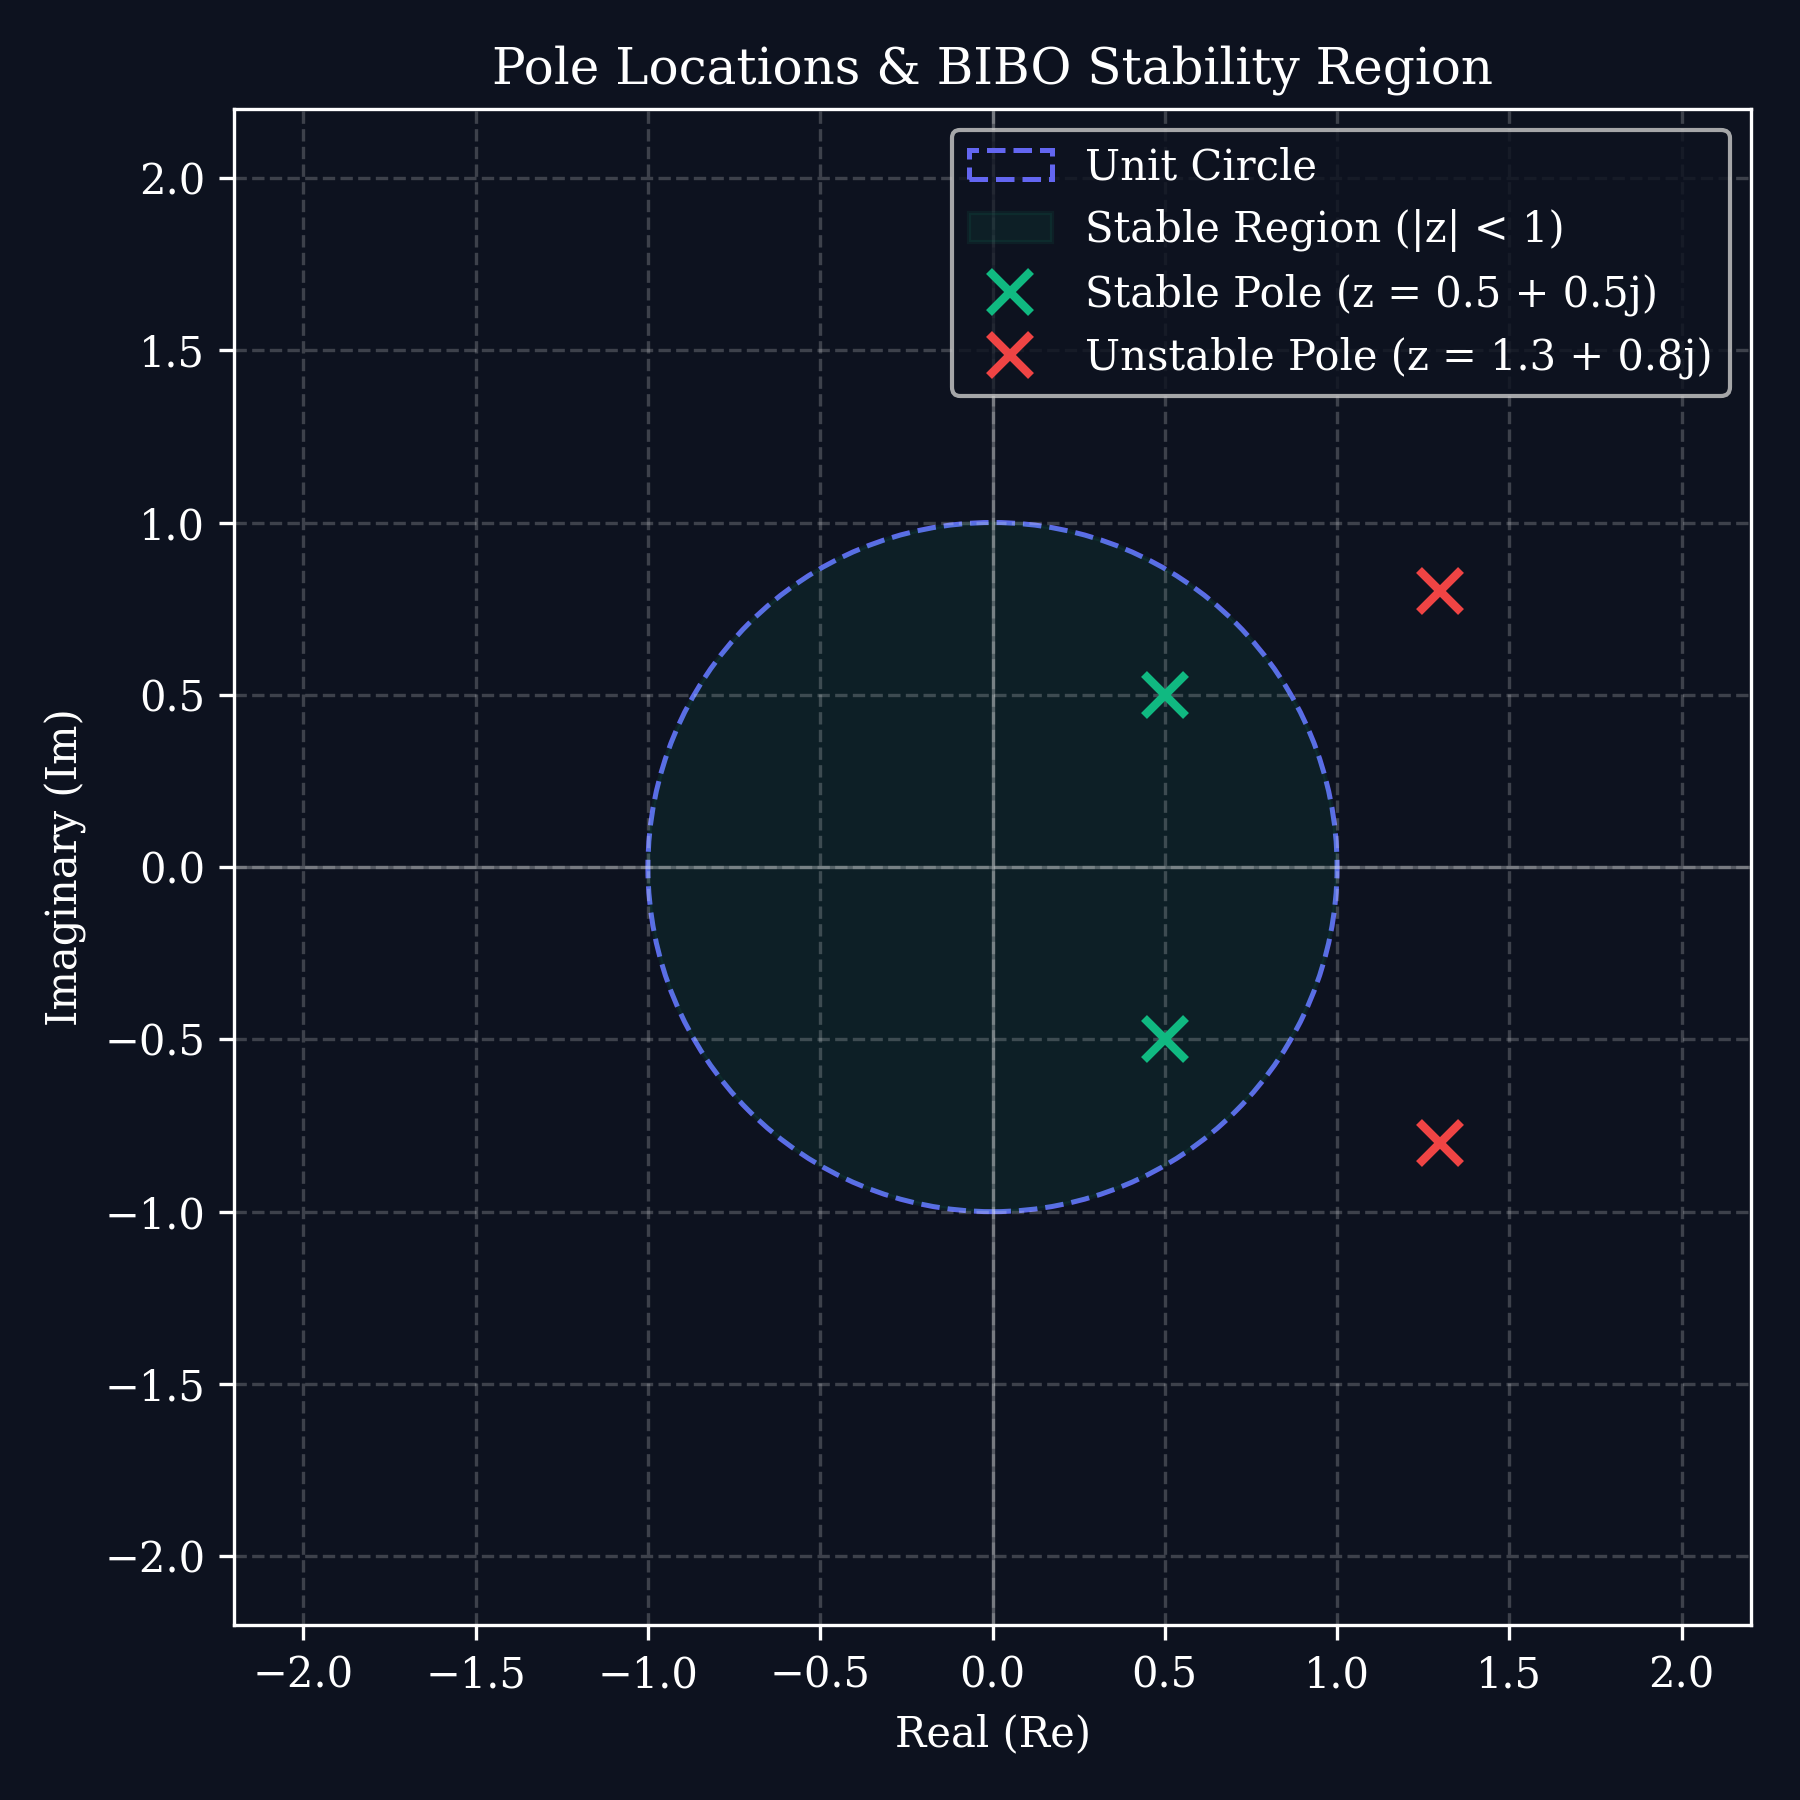
\includegraphics[width=0.65\textwidth]{images/pole_zero_stability_l6.png}
\caption{Stable and unstable pole regions in the z-plane.}
\label{fig:zplane_stability}
\end{figure}

\begin{figure}[H]
\centering
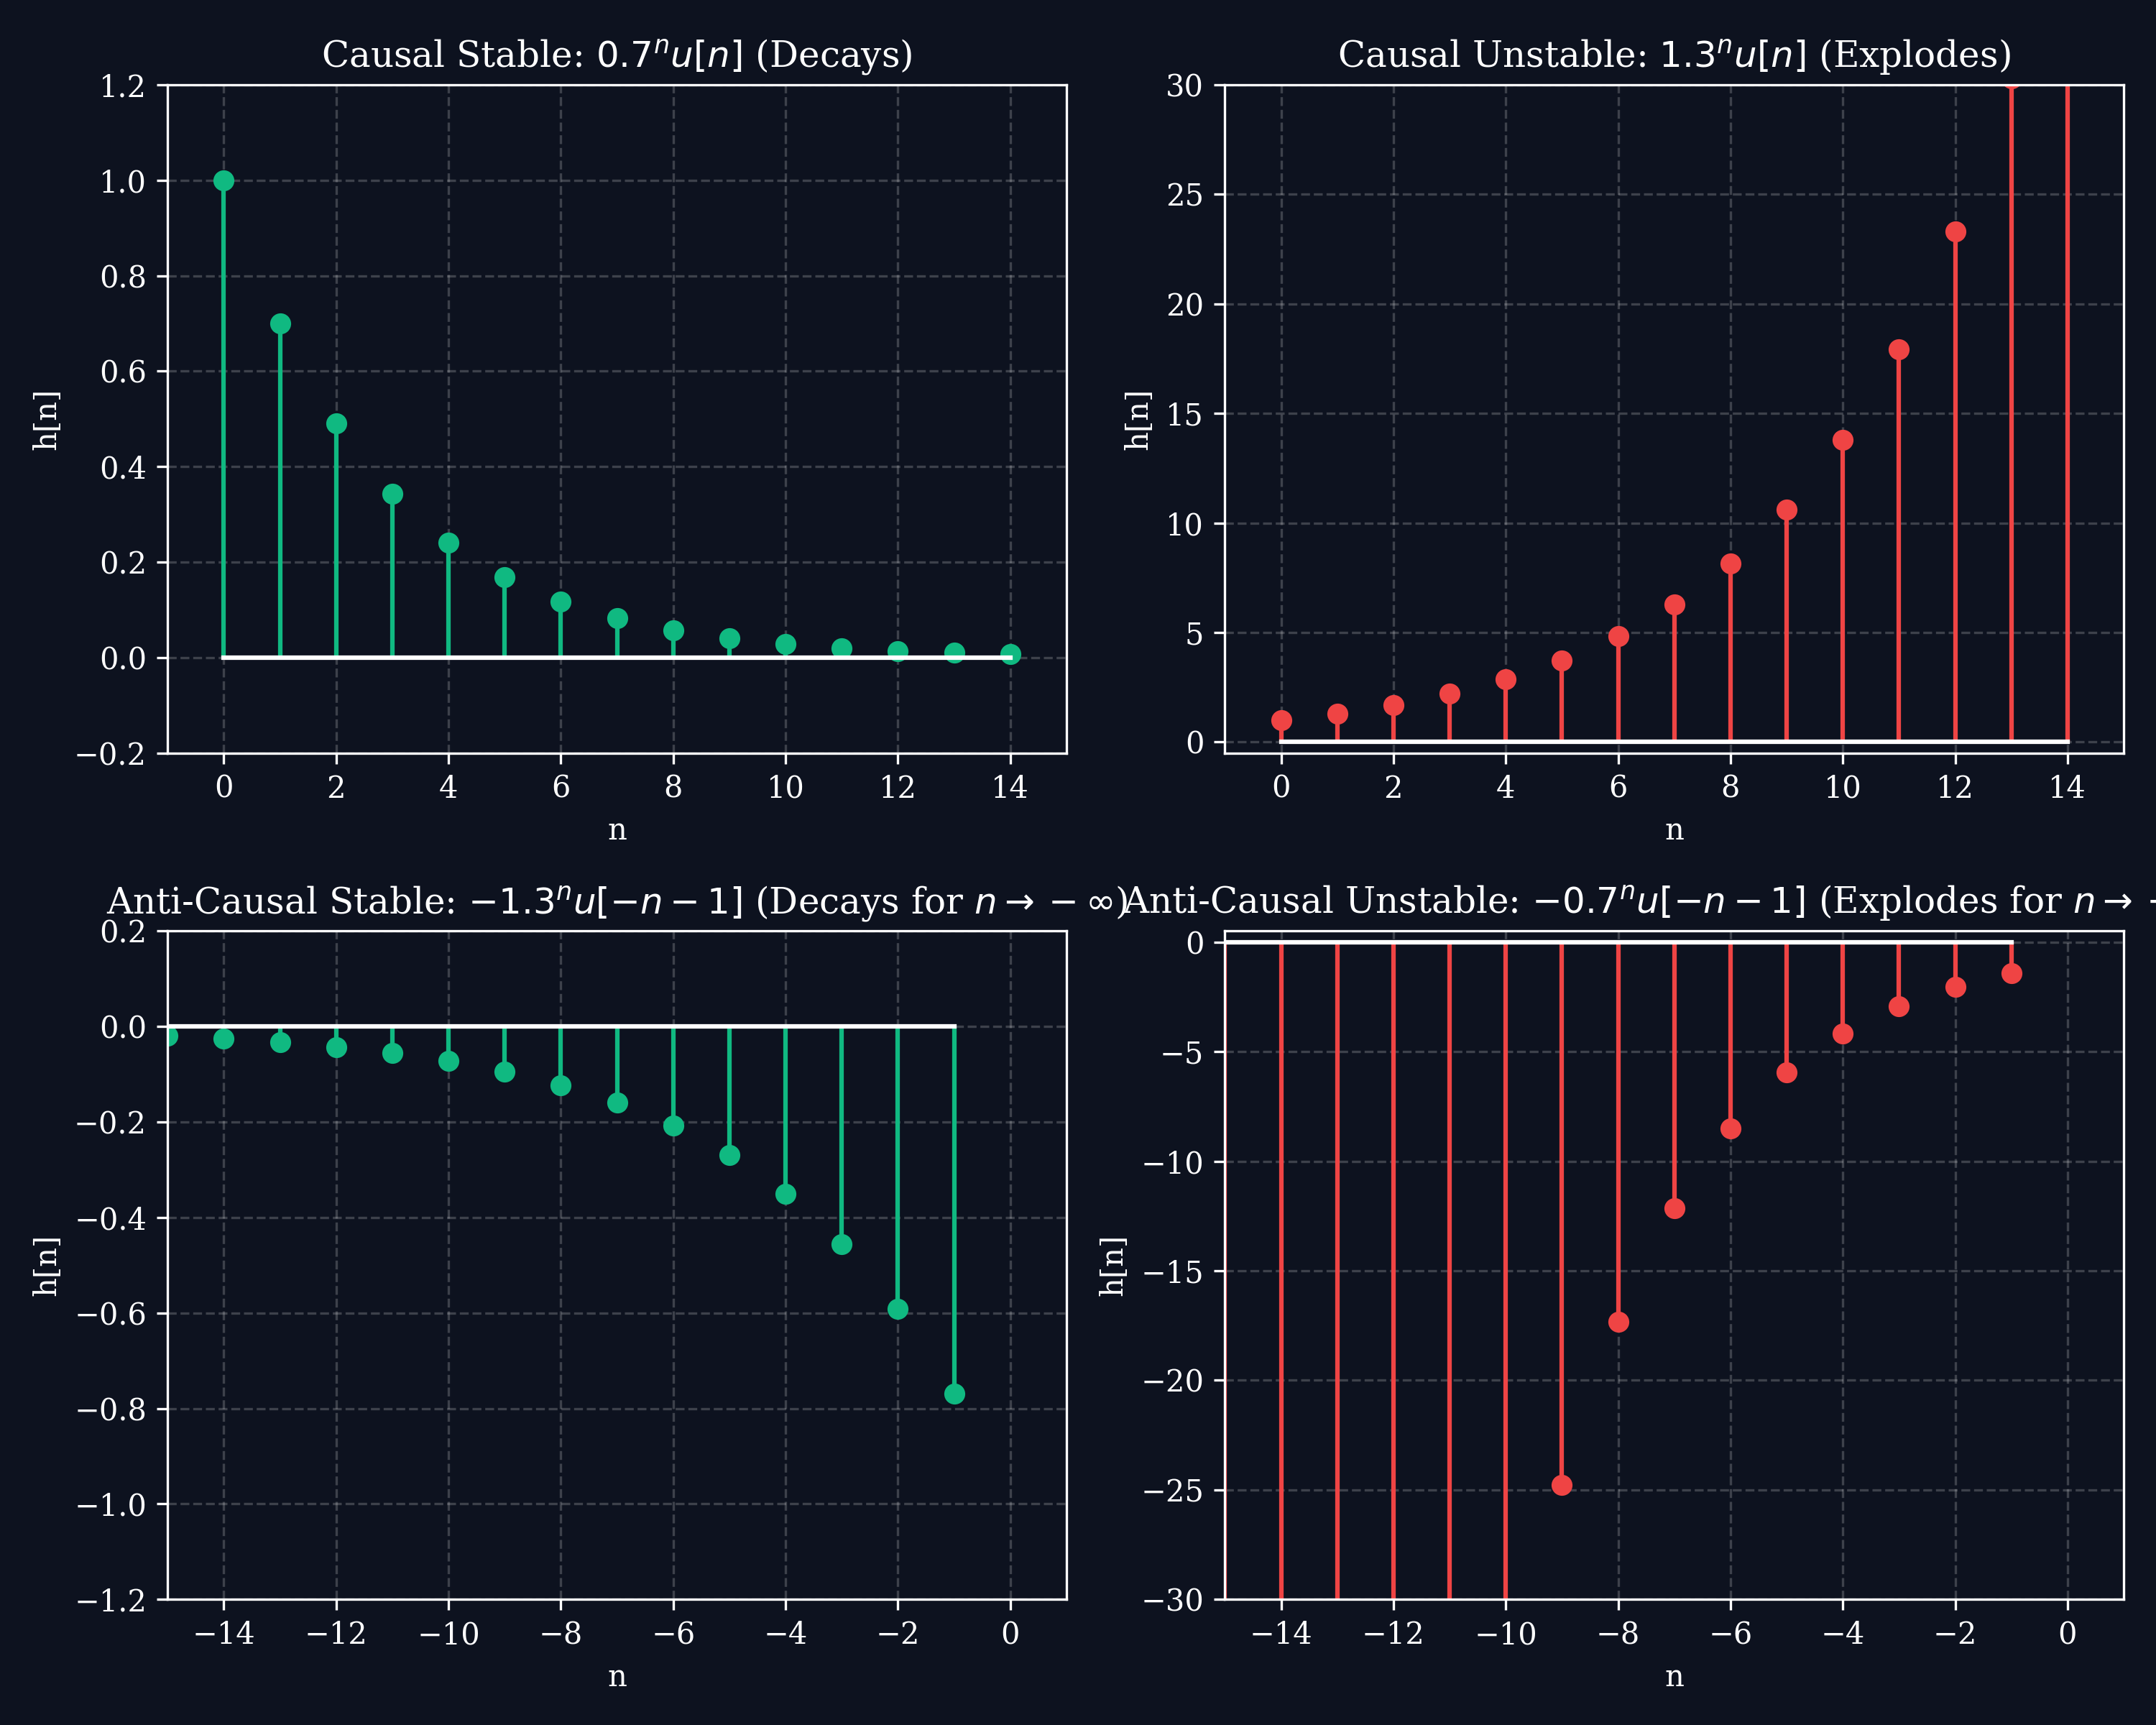
\includegraphics[width=0.85\textwidth]{images/impulse_response_modes.png}
\caption{Decaying (stable) and growing (unstable) impulse response modes.}
\label{fig:impulse_modes}
\end{figure}

\end{document}
